\title{Getting Started}
\documentclass[10pt]{article}
\textwidth 6.5in
\textheight 9in
\oddsidemargin -0.2in
\topmargin -0.5in

\usepackage{graphicx,times,amsmath} % Add all your packages here
\usepackage[all]{xy}
\usepackage{multirow}
\usepackage{graphicx}
\usepackage{color}
\usepackage{tabularx}
\usepackage{url}
\usepackage{amsmath}
\usepackage{amssymb}
\usepackage{multirow}
\usepackage[noend,ruled,linesnumbered]{algorithm2e}
\usepackage[numbers, sort]{natbib}
\usepackage{listings}
\usepackage[svgnames]{xcolor}
%\usepackage{newtxtext}
\definecolor{javared}{rgb}{1,0,0} % for strings
\definecolor{javagreen}{rgb}{0.25,0.5,0.35} % comments
\definecolor{javapurple}{rgb}{0.5,0,0.35} % keywords
\definecolor{javadocblue}{rgb}{0.25,0.35,1} % javadoc
\lstdefinestyle{highlight} {
moredelim=[is][\bfseries\textcolor{javadocblue}]{<<>>}{>><<},
moredelim=[is][\itshape]{!!}{??}
}
\lstset{language=Java,
  keywordstyle=\color{javapurple}\bfseries,
  stringstyle=\color{javared},
  commentstyle=\color{javagreen},
  basicstyle=\tt\small,        % the size of the fonts that are used
                               % for the code
  style=highlight,
  breakatwhitespace=false,         % sets if automatic breaks should only happen at whitespace
  breaklines=true,                 % sets automatic line breaking                   % sets the caption-position to bottom
  extendedchars=true,              % lets you use non-ASCII characters; for 8-bits encodings only, does not work with UTF-8
  showspaces=false,                % show spaces everywhere adding particular underscores; it overrides 'showstringspaces'
  showstringspaces=false,          % underline spaces within strings only
  showtabs=false,                  % show tabs within strings adding particular underscores
  tabsize=2,                     % sets default tabsize to 2 spaces
  numbers=left,
  %frameround=ftff,
  frame=shadowbox,
  rulecolor=\color{black},
  rulesepcolor=\color{gray}
  }
\usepackage{hyperref}
\hypersetup{
    colorlinks=true,
    citecolor=teal,
    linkcolor=olive, % Internal links, those generated by cross-referenced elements    
    urlcolor=blue % Links to web sites
}
\newcommand{\sbol}[1]{\textbf{#1}}

\begin{document}
  \setlength{\parindent}{1em}
  \setlength{\parskip}{0em}
  \setlength{\parsep}{0em}

\noindent In this tutorial, we describe steps for setting up a Maven
project that uses {\tt libSBOLj} in Eclipse. Another tutorial follows this one which explains how we use SBOL
2 to represent the function of a state-of-the-art design, namely a
CRISPR-based repression module Kiani~\textit{et
  al.}~\cite{kiani2014crispr} using the Java library. 

\section*{Set up Maven plugins in Eclipse}
In this section, we describe steps for installing Maven plugins in Eclipse. The Eclipse version used is Luna Service Release 2 (4.4.2). One thing to mention before we start the tutorial is users do need to take note while attempting this tutorial that if any plugins are already installed, then Eclipse won't allow re-installation of that plug-in and any relating steps described within the tutorial can be skipped. Here are the steps:
\begin{enumerate}
\item Versions of Eclipse later than Luna has Maven installed already, therefore users can skip steps to the install Maven plugin and continue to Creating a new project section.
\item In Eclipse, go to Help and select Install New Software,
\item Add a new software site: Name = slf4j, URL = \url{http://www.fuin.org/p2-repository/}, 
\item Check the site specified in previous step to work with, expand Maven osgi-bundles, and select slf4j.api, 
\item Click Next and follow the installation process.

\quad \textbf{Note:} Users may be prompted to restart Eclipse. While it isn't required to restart Eclipse, it is \textbf{recommended} to restart to ensure that the new software was installed.   

\item Add a new software site: Name = Maven Plugins, URL = \url{http://download.eclipse.org/technology/m2e/releases}, 
\item Check the site specified in previous step to work with, expand Maven Integration for Eclipse, and select m2e - Maven Integration for Eclipse, and
\item Click Next and follow the installation process.
\end{enumerate}

\section*{Creating a new project}
After the Maven plugin is installed, we are now ready to create a new Maven project in Eclipse. The following text describe the necessary steps. 

In the package explorer window, right click and select {\bf New $\rightarrow$ Other}.
\begin{center}
  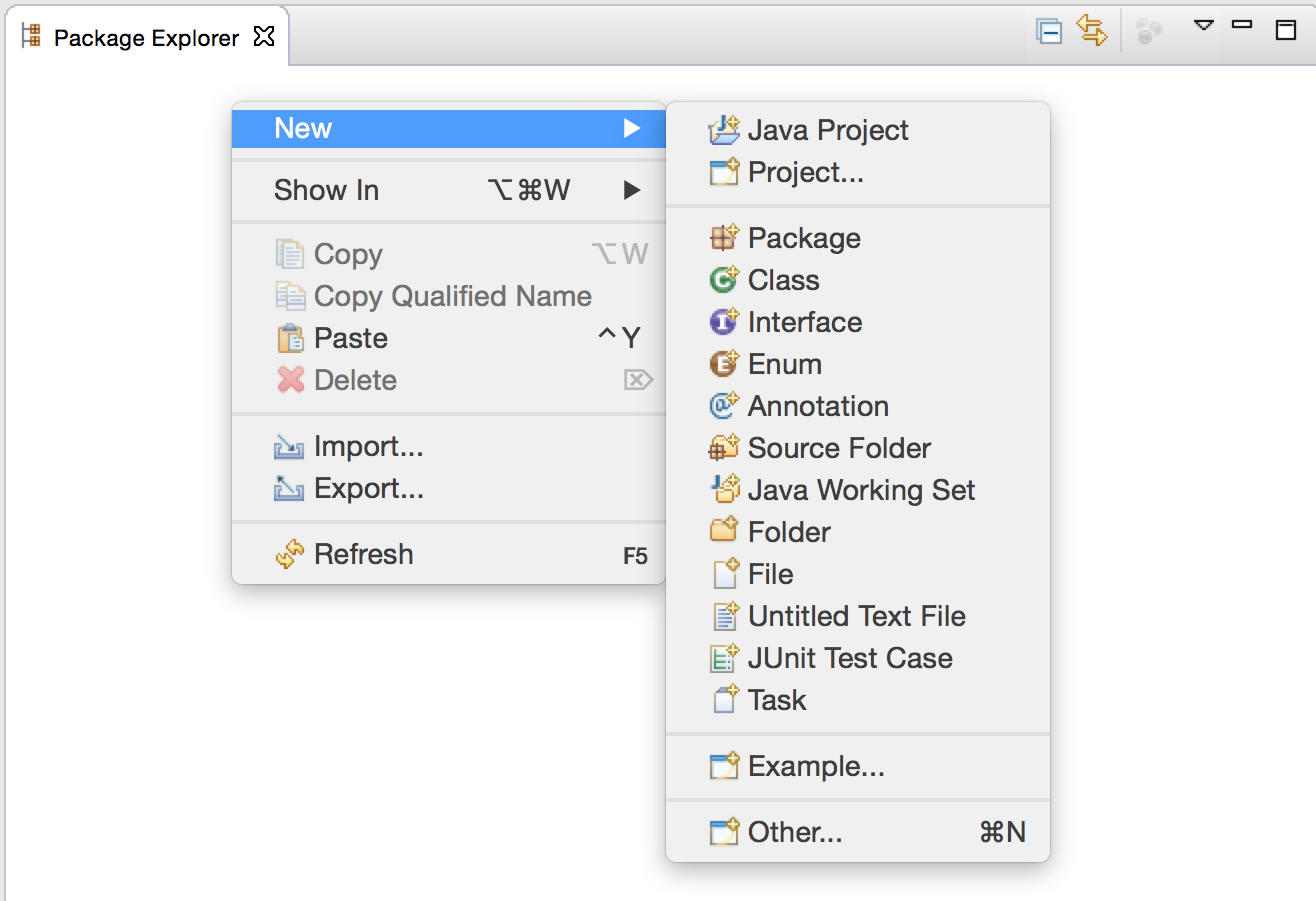
\includegraphics[width=0.8\textwidth]{figures/createNewMavenProject1}
\end{center}

Under the {\bf Maven} folder, choose {\bf Maven Project}, and then follow the default options for the project setup.
\begin{center}
  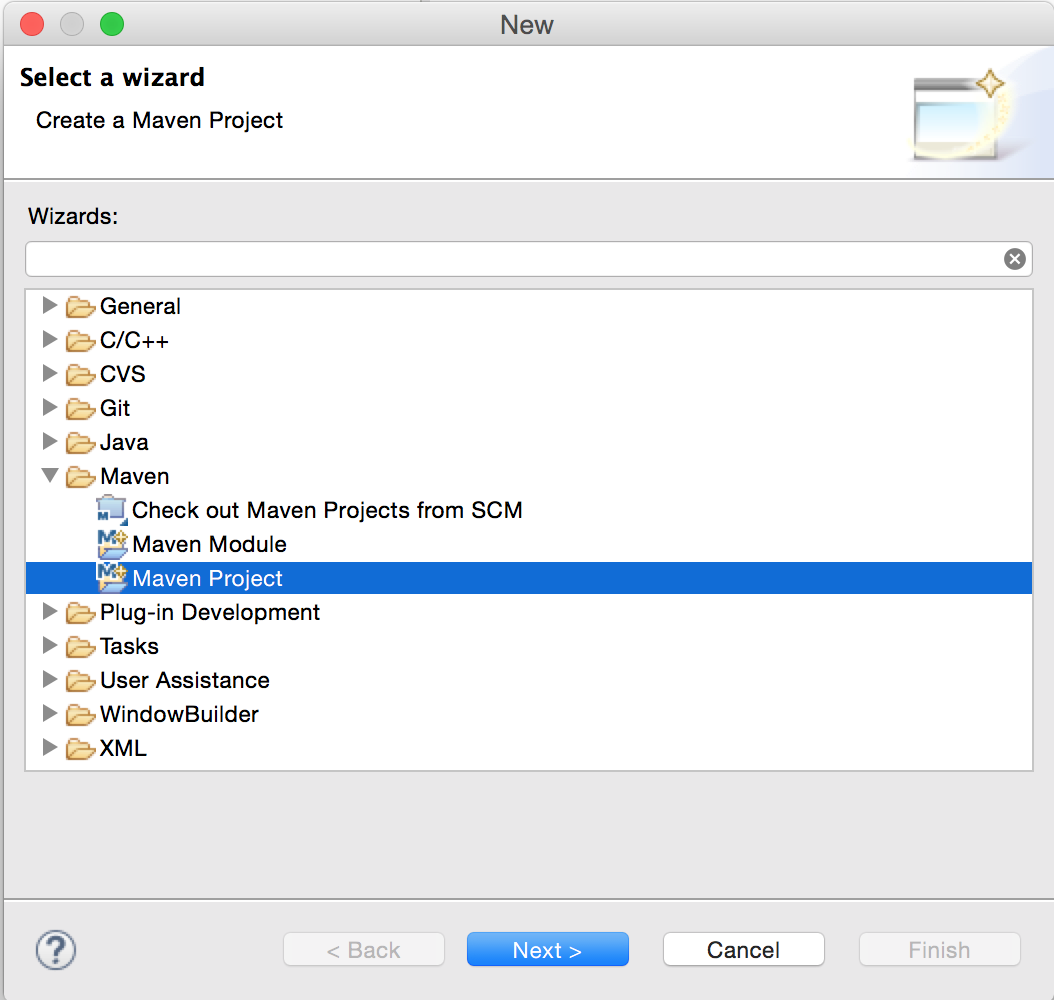
\includegraphics[width=0.75\textwidth]{figures/createNewMavenProject2}
\end{center}

% \begin{center}
%   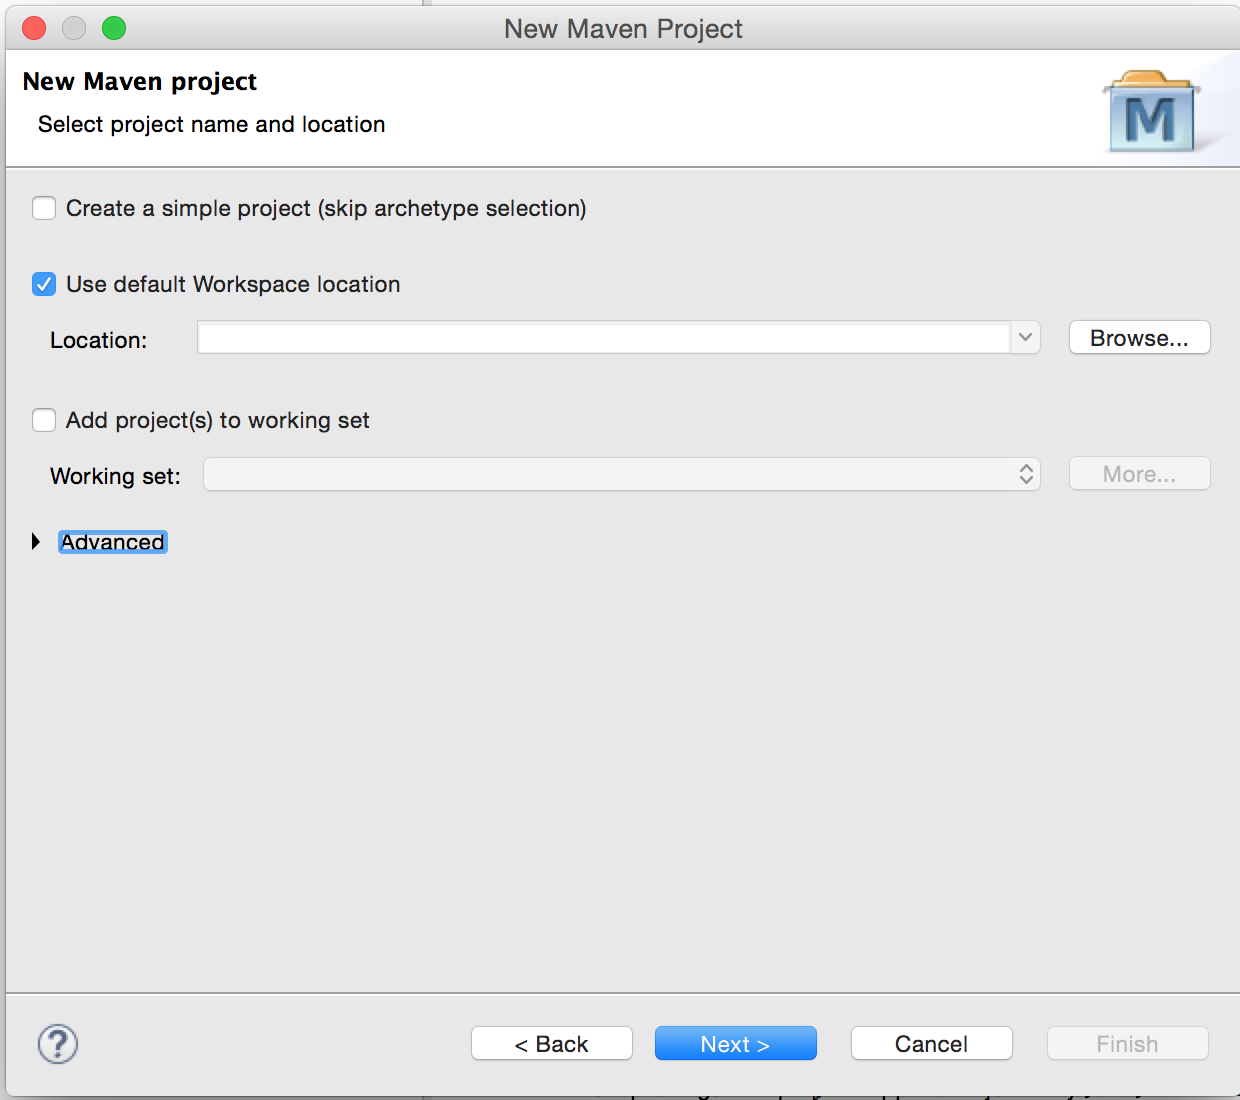
\includegraphics[width=0.8\textwidth]{figures/createNewMavenProject3}
% \end{center}

\begin{center}
  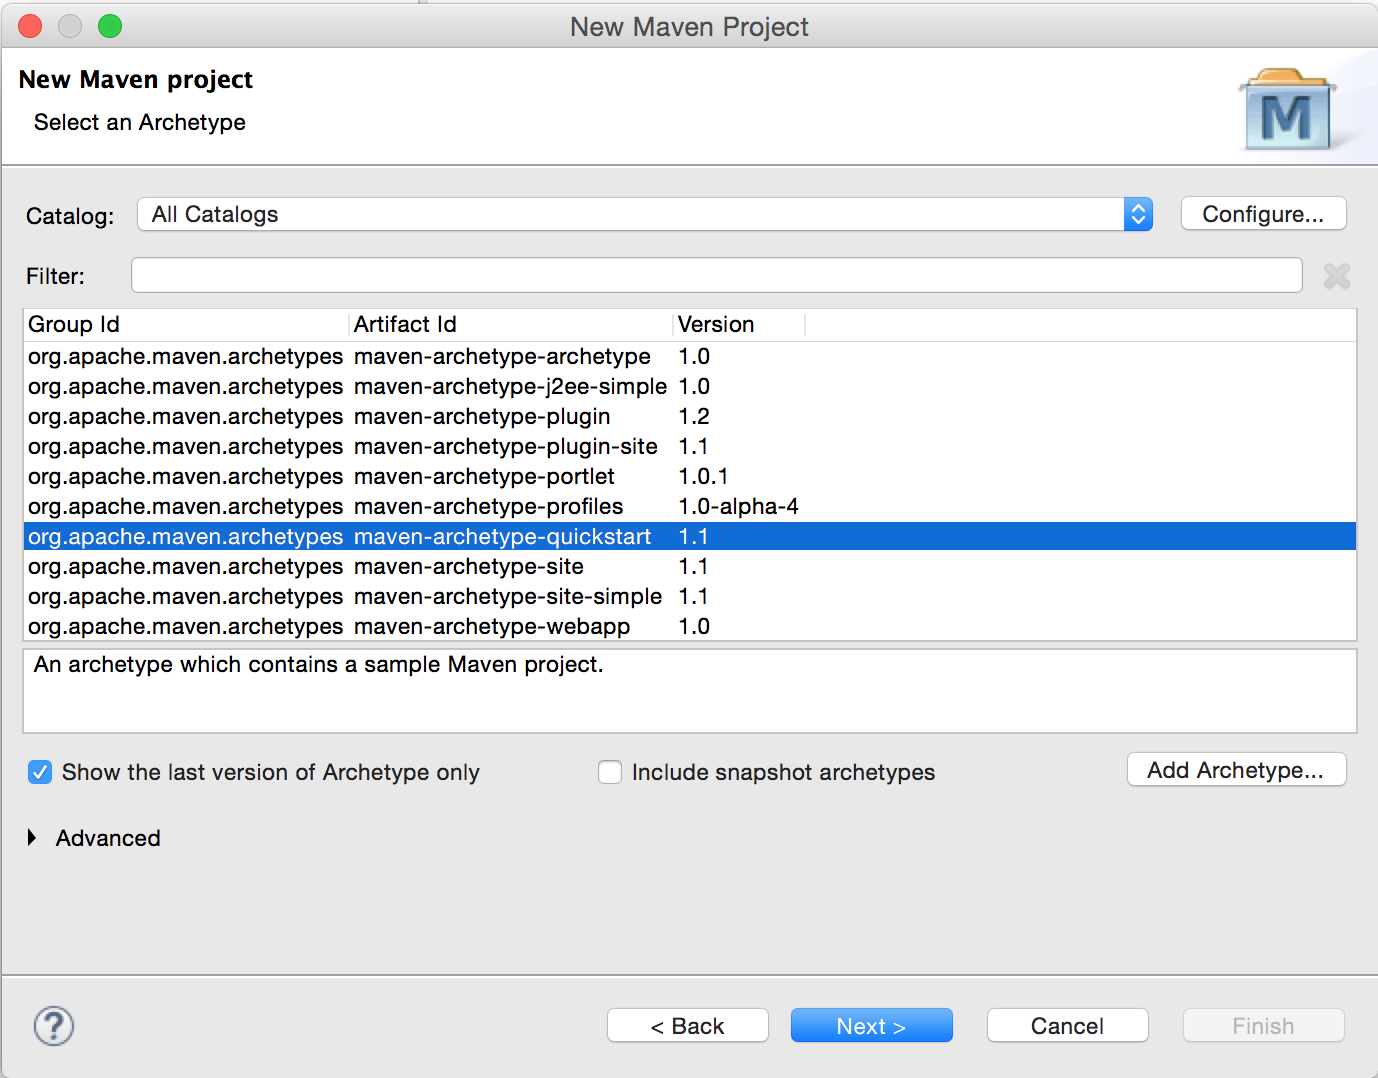
\includegraphics[width=0.75\textwidth]{figures/createNewMavenProject4}
\end{center}

In the window for specifying archetype parameters, you may type your group ID and artifact ID. In this tutorial, they are specified as shown below. 
\begin{center}
  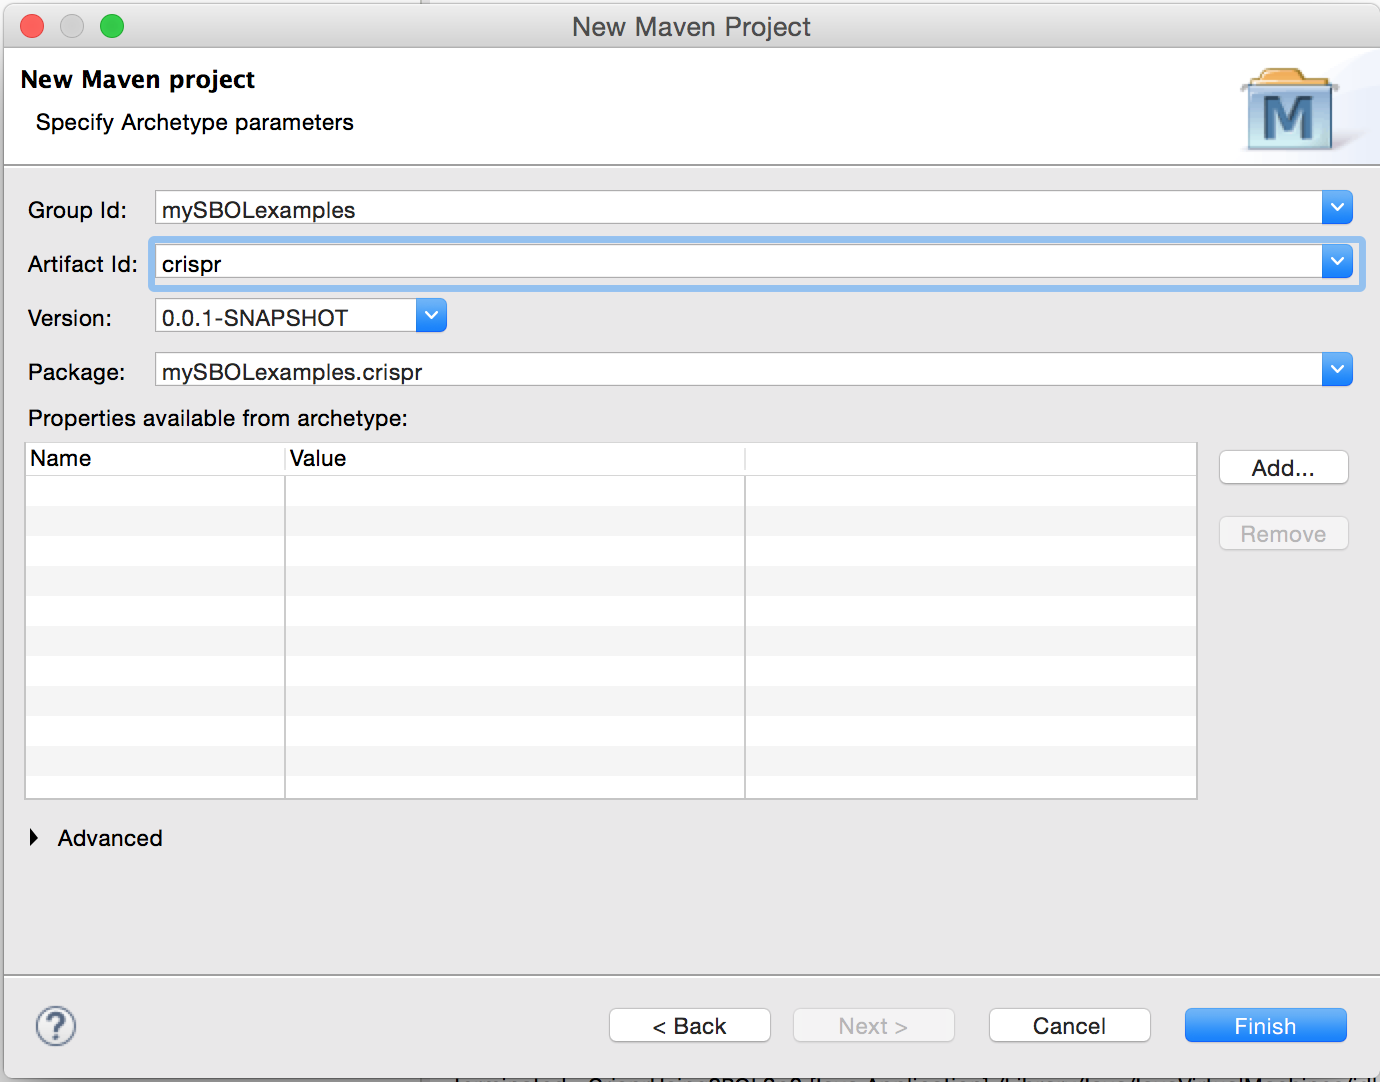
\includegraphics[width=0.8\textwidth]{figures/createNewMavenProject5}
\end{center}

Once the project setup is finished, you should be able to see two Java source folders, a {\bf JRE System Library} and a {\bf Maven Dependencies} library, and a {\bf pom.xml} file. 
\begin{center}
  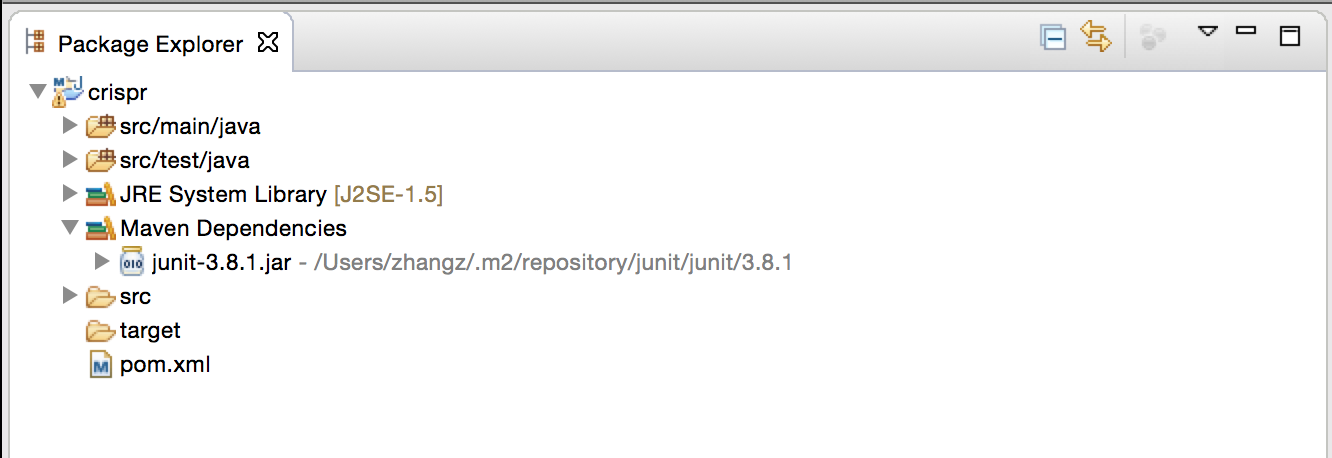
\includegraphics[width=0.8\textwidth]{figures/createNewMavenProject6}
\end{center}

It is possible that the JRE System Library created by Maven is not compatible with the installed JREs. In the screenshot shown below, it is set to {\bf J2SE-1.5}, but the Maven compiler is compatible with {\bf JavaSE-1.7} instead. To change it, right-click on the ``crispr'' project and then select {\bf Maven $\rightarrow$  Update Project}, the JRE will reset itself back to J2SE-1.5. 
\begin{center}
  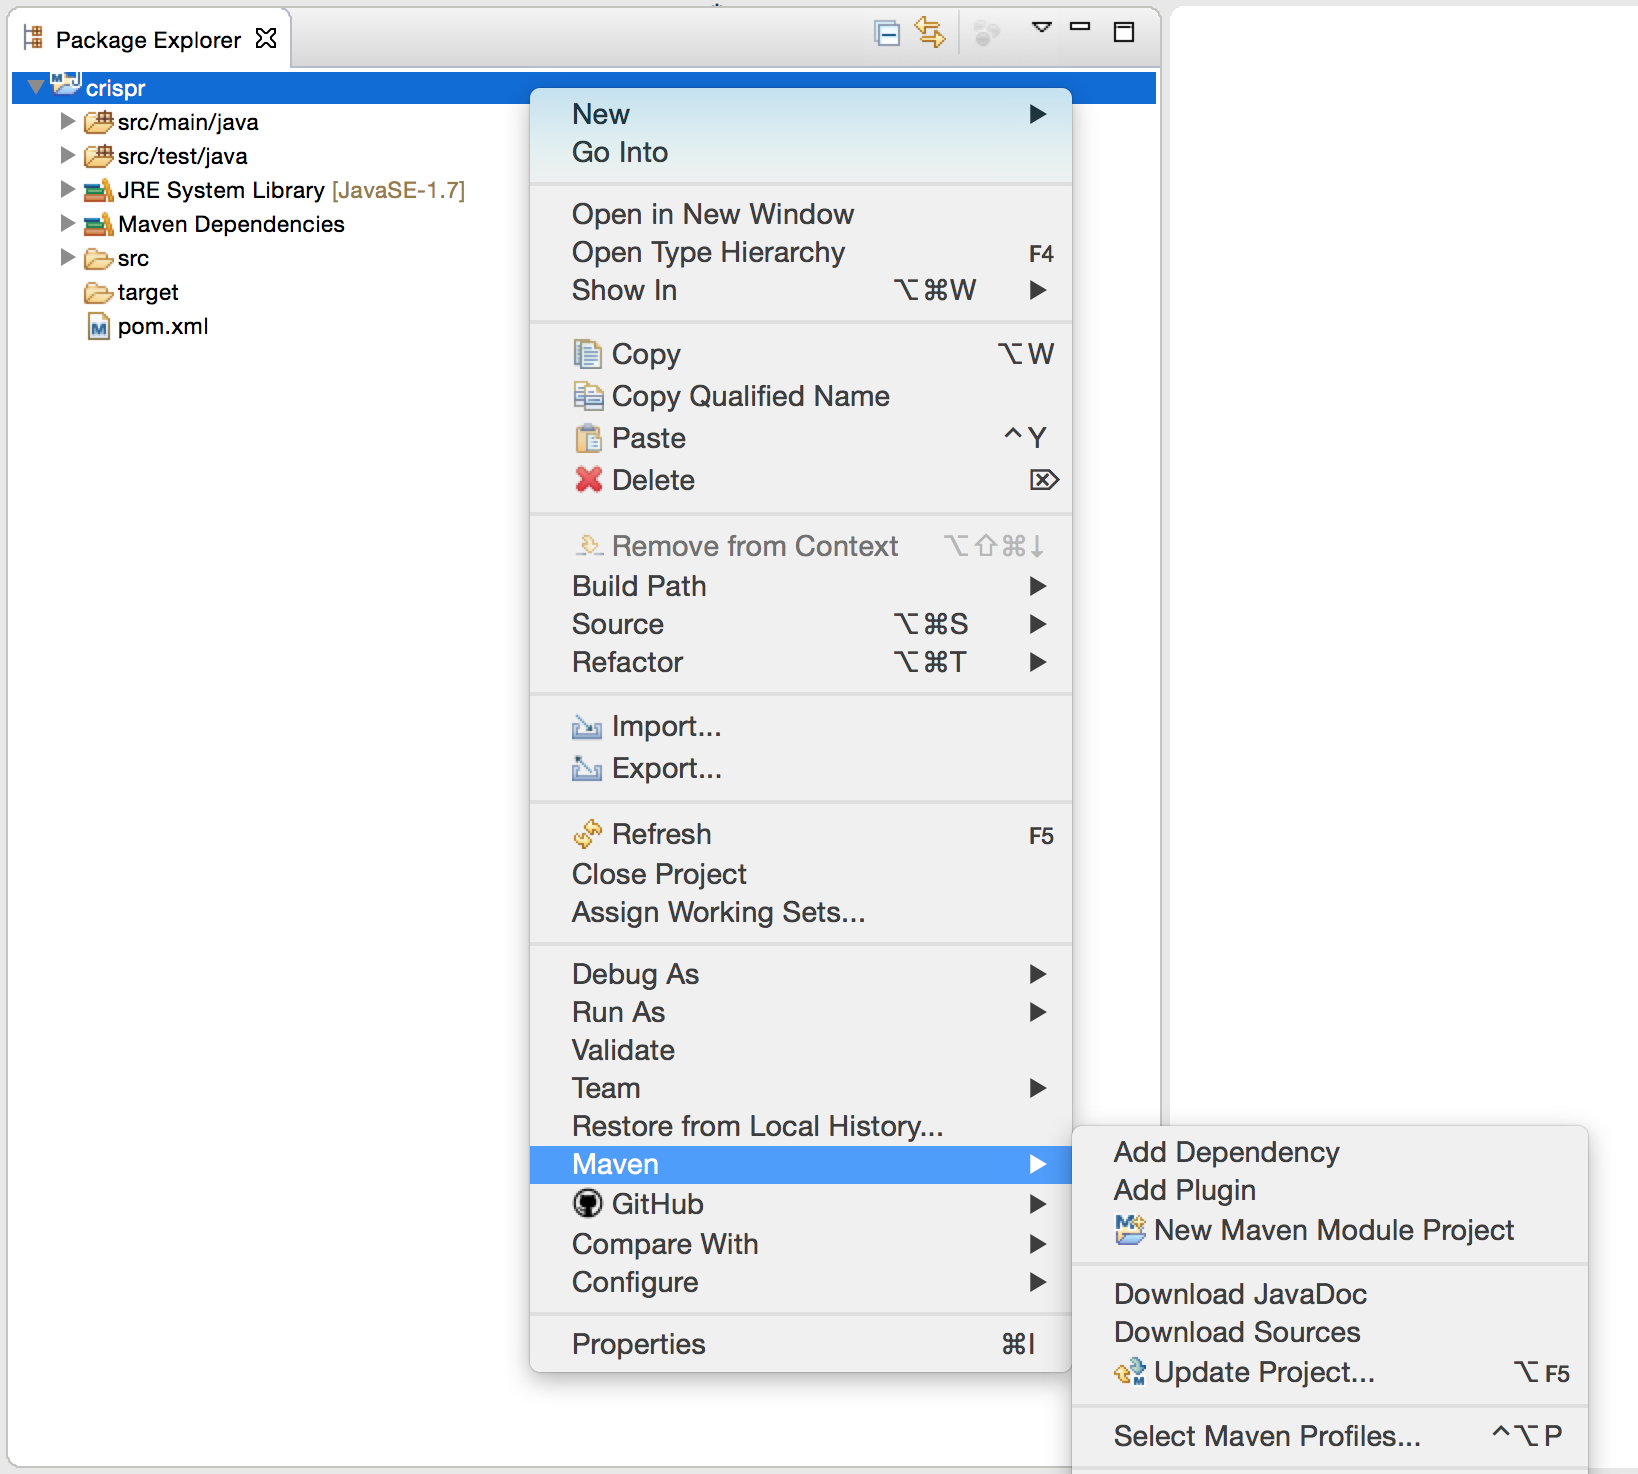
\includegraphics[width=0.8\textwidth]{figures/createNewMavenProject10}
\end{center}

A permanent fix would be to manually add the plugin management information below to the pom.xml file. To access the pom.xml file, the user needs to double-click on the pom.xml file in the project menu. Then once a window pops up, select the rightmost tab on the bottom of the screen titled {\bf pom.xml}. 

\begin{minipage}{\textwidth}
\pagestyle{empty}
\begin{lstlisting}
[language=xml,basicstyle=\footnotesize\ttfamily]
<build>
    <pluginManagement>
        <plugins>
            <plugin>
                <groupId>org.apache.maven.plugins</groupId>
                <artifactId>maven-compiler-plugin</artifactId>
                <version>3.1</version>
                <configuration>
                    <source>1.7</source>
                    <target>1.7</target>
                </configuration>
            </plugin>
        </plugins>
    </pluginManagement>
</build>
\end{lstlisting}
\pagestyle{empty}
\end{minipage}

The pom.xml should look like the one shown below after this modification. Remember to save the file and then do {\bf Maven $\rightarrow$  Update Project}.

\begin{minipage}{\textwidth} 
\lstinputlisting[language=xml,basicstyle=\footnotesize\ttfamily]{pom.xml}
\end{minipage}

\section*{Adding {\tt libSBOLj} as dependency}
We are now ready to add libSBOLj as a Maven dependency. This can be easily done by right-clicking on the ``crispr'' project and then select {\bf Maven $\rightarrow$ Add Dependency}.
% \begin{center}
%   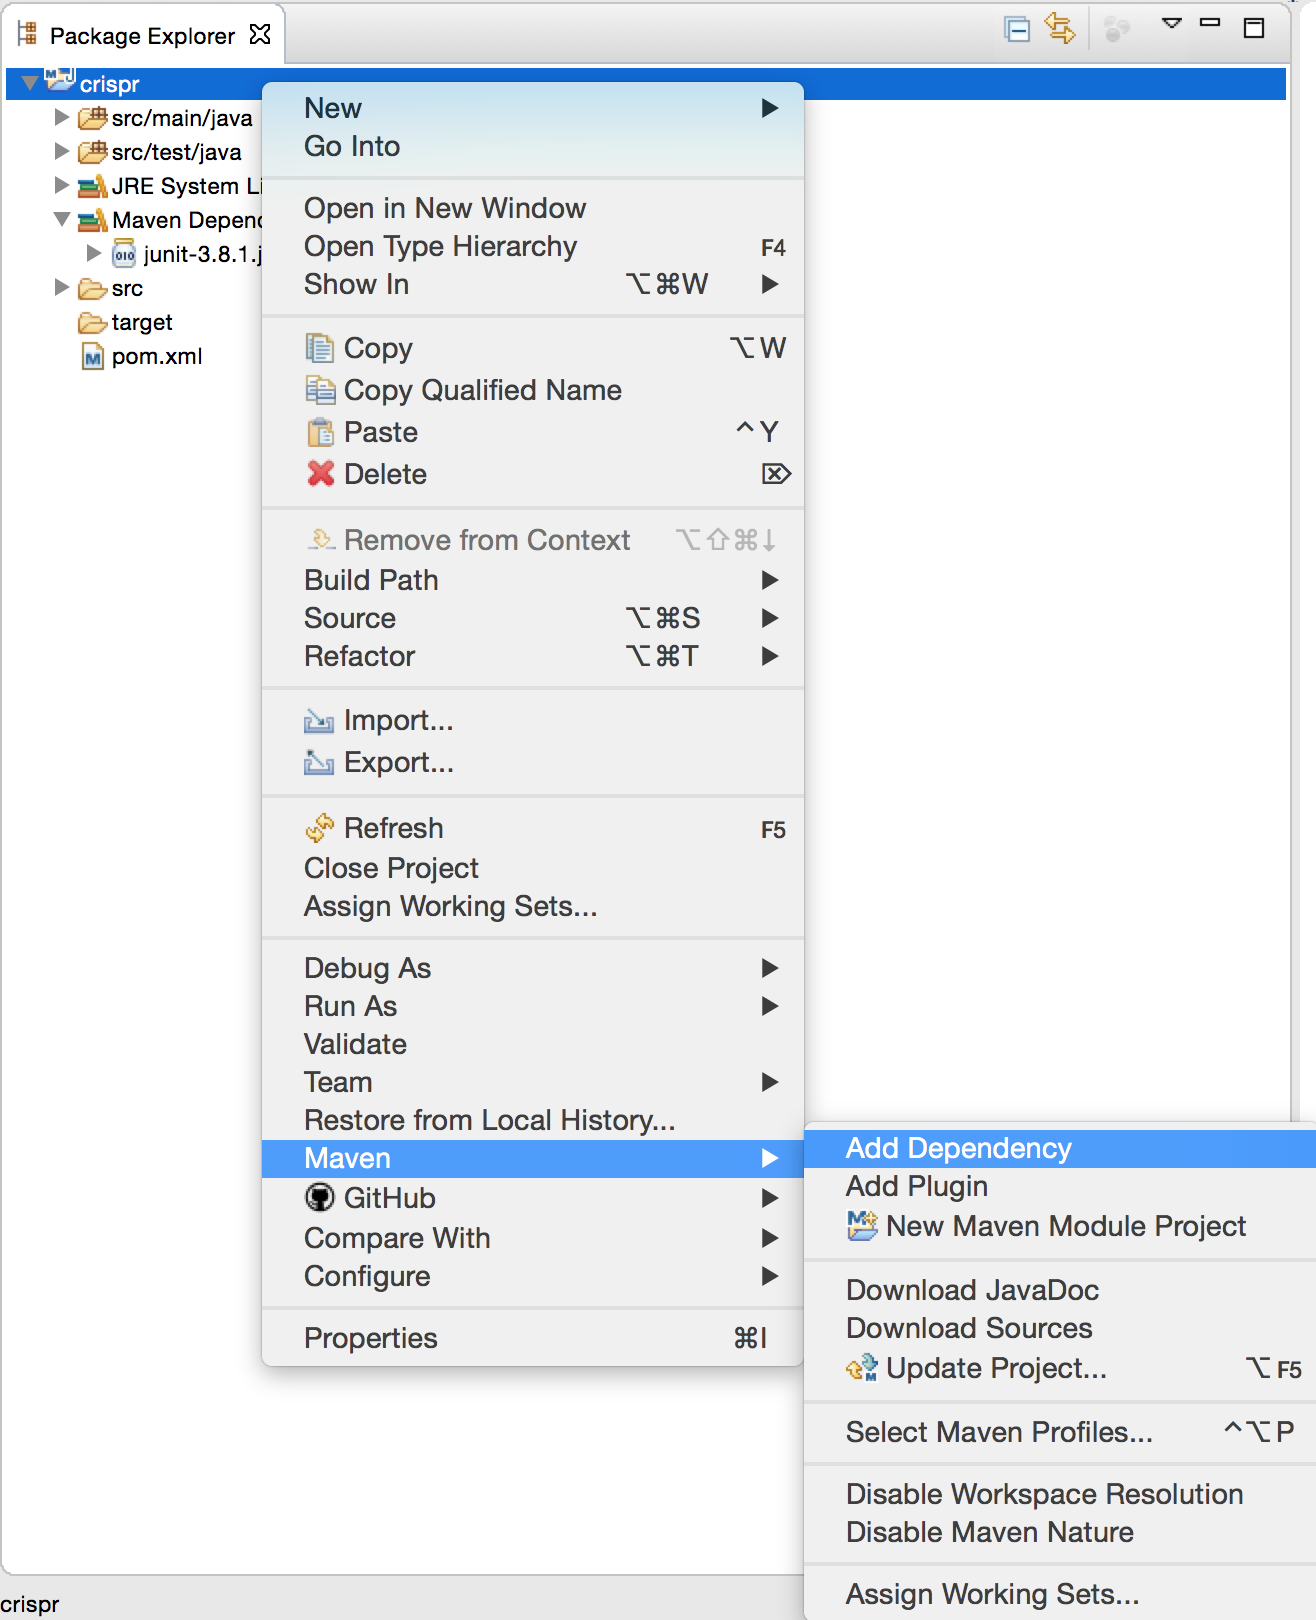
\includegraphics[width=0.55\textwidth]{figures/addMavenDependency1}
% \end{center}
In the popup window shown below, fill in the information for the {\tt libSBOLj} library. The group ID is {\bf org.sbolstandard}, and the artifact ID is {\bf libSBOLj} and the version is {\bf 2.2.1}. 
\begin{center}
  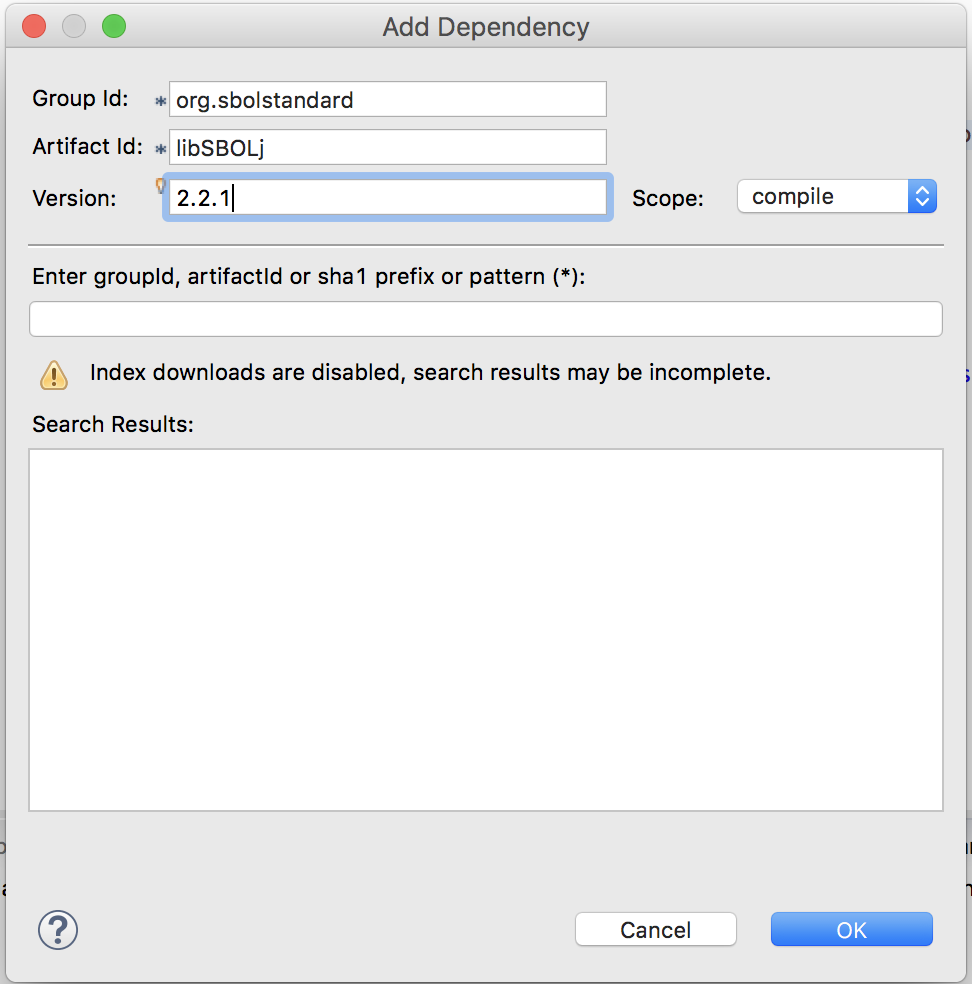
\includegraphics[width=0.55\textwidth]{figures/addMavenDependency2}
\end{center}

After this dependency is added, Maven automatically brings in the  {\tt libSBOLj-2.2.1.jar} and its dependencies from the Maven Central Repository, and places them under the {\bf Maven Dependencies} directory. The user will need to right click on the project directory and select {\bf Maven $\rightarrow$ Update Project}. Within this window, the user needs to ensure that {\bf Force Update of Snapshots/Releases} is checked. 





\bibliographystyle{ieeetr}
\bibliography{top}


\end{document}
